\documentclass{article}
\usepackage{amsmath, amssymb, amsfonts, amsthm}
\usepackage{graphicx}
\usepackage{hyperref}
\usepackage{tikz}
\usepackage{tikz-qtree}
\usepackage[margin=2.5cm]{geometry}


\newtheorem{Corollary}{Corollary}
\newcommand{\classX}[1]{\ensuremath{\text{\textsf{\textbf{#1}}}}} 
\newcommand{\classP}{\classX{P}}
\newcommand{\classNP}{\classX{NP}}
\newcommand{\NPC}{\classX{NP-complete}}
\newcommand{\coNP}{\classX{coNP}}
\newcommand{\EXP}{\classX{EXP}}
\newcommand{\coEXP}{\classX{coEXP}}
\newcommand{\PSPACE}{\classX{PSPACE}}
\newcommand{\NPH}{\classX{NP-hard}}

\newcommand{\MAD}{\ensuremath{\text{\textit{MAD}}}}
\newcommand{\Prob}[1]{\ensuremath{\text{\textsc{#1}}}}

\newtheorem{theorem}{Theorem}
\newtheorem{lemma}{Lemma}
\newtheorem{proposition}{Proposition}

\begin{document}

\title{A meta-heuristic approach for graph genus problem}
\author{Syed Mujtaba Hassan\footnote{\url{ms06948@st.habib.edu.pk}, Computer Science Department, Habib University, Karachi, Pakistan} \and Sudais Yasin \footnote{\url{sy06541@st.habib.edu.pk}, Computer Science Department, Habib University, Karachi, Pakistan}}
\date{May 8, 2024}
\maketitle


\begin{abstract}

    \noindent\textbf{Keywords:} graph theory, graph genus, algebraic topology, evolutionary algorithms
\end{abstract}


\renewcommand\thefootnote{}


\renewcommand\thefootnote{\fnsymbol{footnote}}
\setcounter{footnote}{1}
\section{Introduction}\label{sec1}
    Graph genus problem can be dated back to the map coloring problem proposed in 1890 by Heawood \cite{Liangxia23}.
    Intuitively the problem is to draw a graph on an orientable surface with $n$ holes without any edges crossing. 
    The minimum number of holes any such surface can have is known as the genus of the graph. The genus of a graph is the primary criterion of non-planarity.
    The genus problem is known to be $\NPH$ \cite{Thomassen89}. The problem is known to be $\NPH$ even for cubic graphs \cite{Thomassen97}.
    The problem is one of the hardest problems in graph theory and algebraic topology. Furthermore, the problem has a higher complexity even for smaller graphs. The brute force approach run in $O(|V|^{\Delta(G)})$ time. 
    Despite the hardness of the problem, there are several real-world applications of the genus problem, such as utility problem, and circuit embedding, among others.

    We introduce a meta-heuristic approach for the graph genus problem. We apply an evolutionary algorithm (EA) to approximate a solution to the graph genus problem. 
    This is the meta-heuristic approach to the genus problem. In section~\ref{sec: prelim} we shall introduce our definitions and the problem more formally.
    In section~\ref{sec: EA} we give an EA formulation of our graph genus problem. Our formulation and algorithm are then experimentally evaluated in section~\ref{sec: exp}.

   

\section{Topologic and graph theoretic preliminaries}\label{sec: prelim}
    We first need to go over some graph theoretic and topological prerequisites.
    Throughout this document, we will denote a graph as $G = (V, E)$ where $G$ is a graph with vertex set $V$ and edge set $E$. An edge is represented as a set $\{v, u\}$ for some $v$ and $u$ belonging to $V$ such that $v \neq u$. Also, for a graph $G$ we use $V(G)$ to denote the vertex set of $G$ and $E(G)$ to denote the edge set of $G$. 
    Unless specified, all graphs considered here are undirected and simple meaning they contain no loops, multi-edges or directed edges. 
    For each vertex $v\in V$ we used $d_G(v)$ to denote the degree of $v$ in $G$. We also use $\Delta(G)$ to denote the maximum degree of $G$ and $\delta(G)$ to denote the minimum degree of $G$. 
    An isomorphism between graphs $G = (V, E)$ and $G' = (V', E')$ is a bijection $f : V \to V'$ such that $\forall v, u \in V,\; \{v, u\} \in E \iff  \{f(v), f(u)\} \in E'$ \cite{Diestel97, West01}. For a vertex $v \in V$, $N(v)$ denotes the set of neighbors of $v$ \cite{Diestel97}. 
    For a graph $G = (V, E)$, $D(G)$ denotes the directed graph obtained from $G$ such that 
    A rotation at a vertex $v$ is a cyclic order (counter-clockwise) of the neighbors of $v$. A rotation system $R$ of a graph $G$ is a set of rotations for each vertex $v \in V$ \cite{Beyer16}.
    A directed graph is a graph $G  = (V, E)$ where edges have direction, so an edge from $v$ to $u$ is represented as $(v, u)$, for $v,u \in V$. In a directed graph for a vertex $v \in V$, $d^+(v)$ denotes the out going edges of $v$ and $d^-(v)$ incoming edges on $v$.
    % We shall use the terms ``abstract graph'' and ``graph'' interchangeably, whenever we use the term ``graph'' we are referring to an abstract graph.

    We shall denote a surface $X$, by topological space $(X, \tau)$, where $X$ is a the set topology is defined on and $\tau$ is the topology on $X$. 
    A homeomorphism between two topological spaces is a continuous bijective map whose inverse is also continuous \cite{Munkres00}.
    An $n$-manifolds is a Hausdorff space such that each point has an open neighborhood homeomorphic to the open $n$-dimensional disc $U^n =  \{x \in R^n\mid \; |x| < 1\}$ \cite{Massey91}.
    A connected $2$-manifold is said to be orientable if every closed path is orientation preserving (traversing the path does not change the orientation) \cite{Massey91}.
    Now we shall restrict the surfaces we deal with further. Here the surfaces we deal with are orientable, compact and connected $2$-manifolds.
    Also, we only consider $R^3$ under the usual topology, so we are dealing only with subspaces of $R^3$ under the usual topology.
    Intuitively a Torus is a surface homeomorphic to a donut or a coffee mug. Formally, a torus is any topological space homeomorphic to the product space of two circles in $R^2$, $S^1 \times S^1$ \cite{Massey91}. 
    In other words, a torus is any topological space homeomorphic to the subset $T = \{(x, y, z)\in R^3\mid \; (\sqrt{x^2 + y^2} - 2)^2 + z^2 = 1 \}$ of $R^3$ \cite{Massey91}. There are many equivalent formal definitions of a torus we presented two of the easiest ones here.
    Figure~\ref*{Fig2} shows an example of a torus.
    \begin{figure}[h]
        \centering
        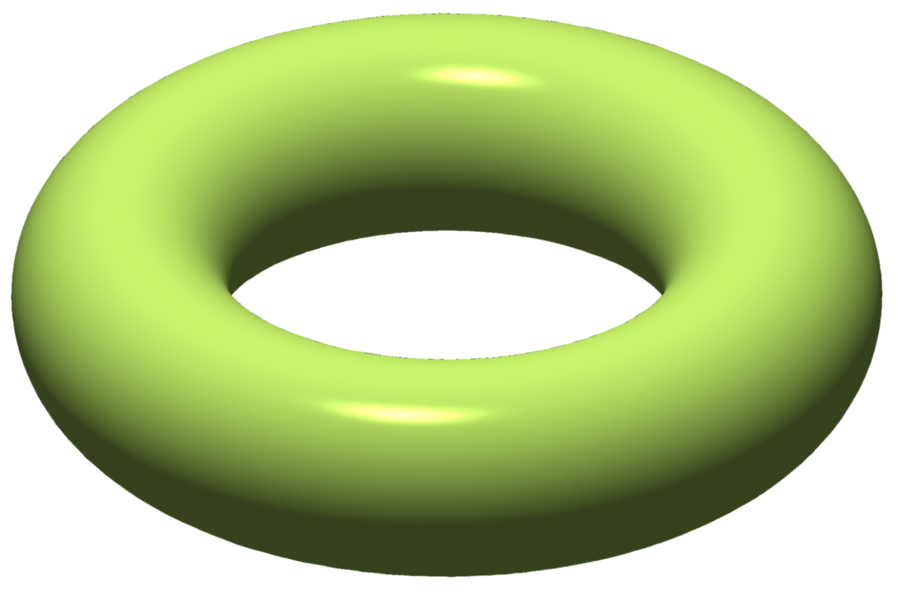
\includegraphics[scale = 1]{Torus_illustration.png} 
        \caption{Torus}
        \label{Fig2}
    \end{figure}
    For two surfaces $S_1$ and $S_2$, their connected sum is a surface $S$, denoted by $S_1 \# S_2$, which is obtained by cutting a small circular hole in each surface, and then gluing the two surfaces together along the boundaries of the holes \cite{Massey91}.
    A surface that is the connected sum of $n$ tori has a genus $n$. Intuitively this means the surface has $n$ holes \cite{Massey91}. Figure~\ref{Fig3} shows two examples of surfaces with genera 2 and 3. Genus of a sphere is defined to be 0.


    \begin{figure}[h]
        \centering
        
\includegraphics[scale = 0.8]{Double_torus_illustration.png} 
        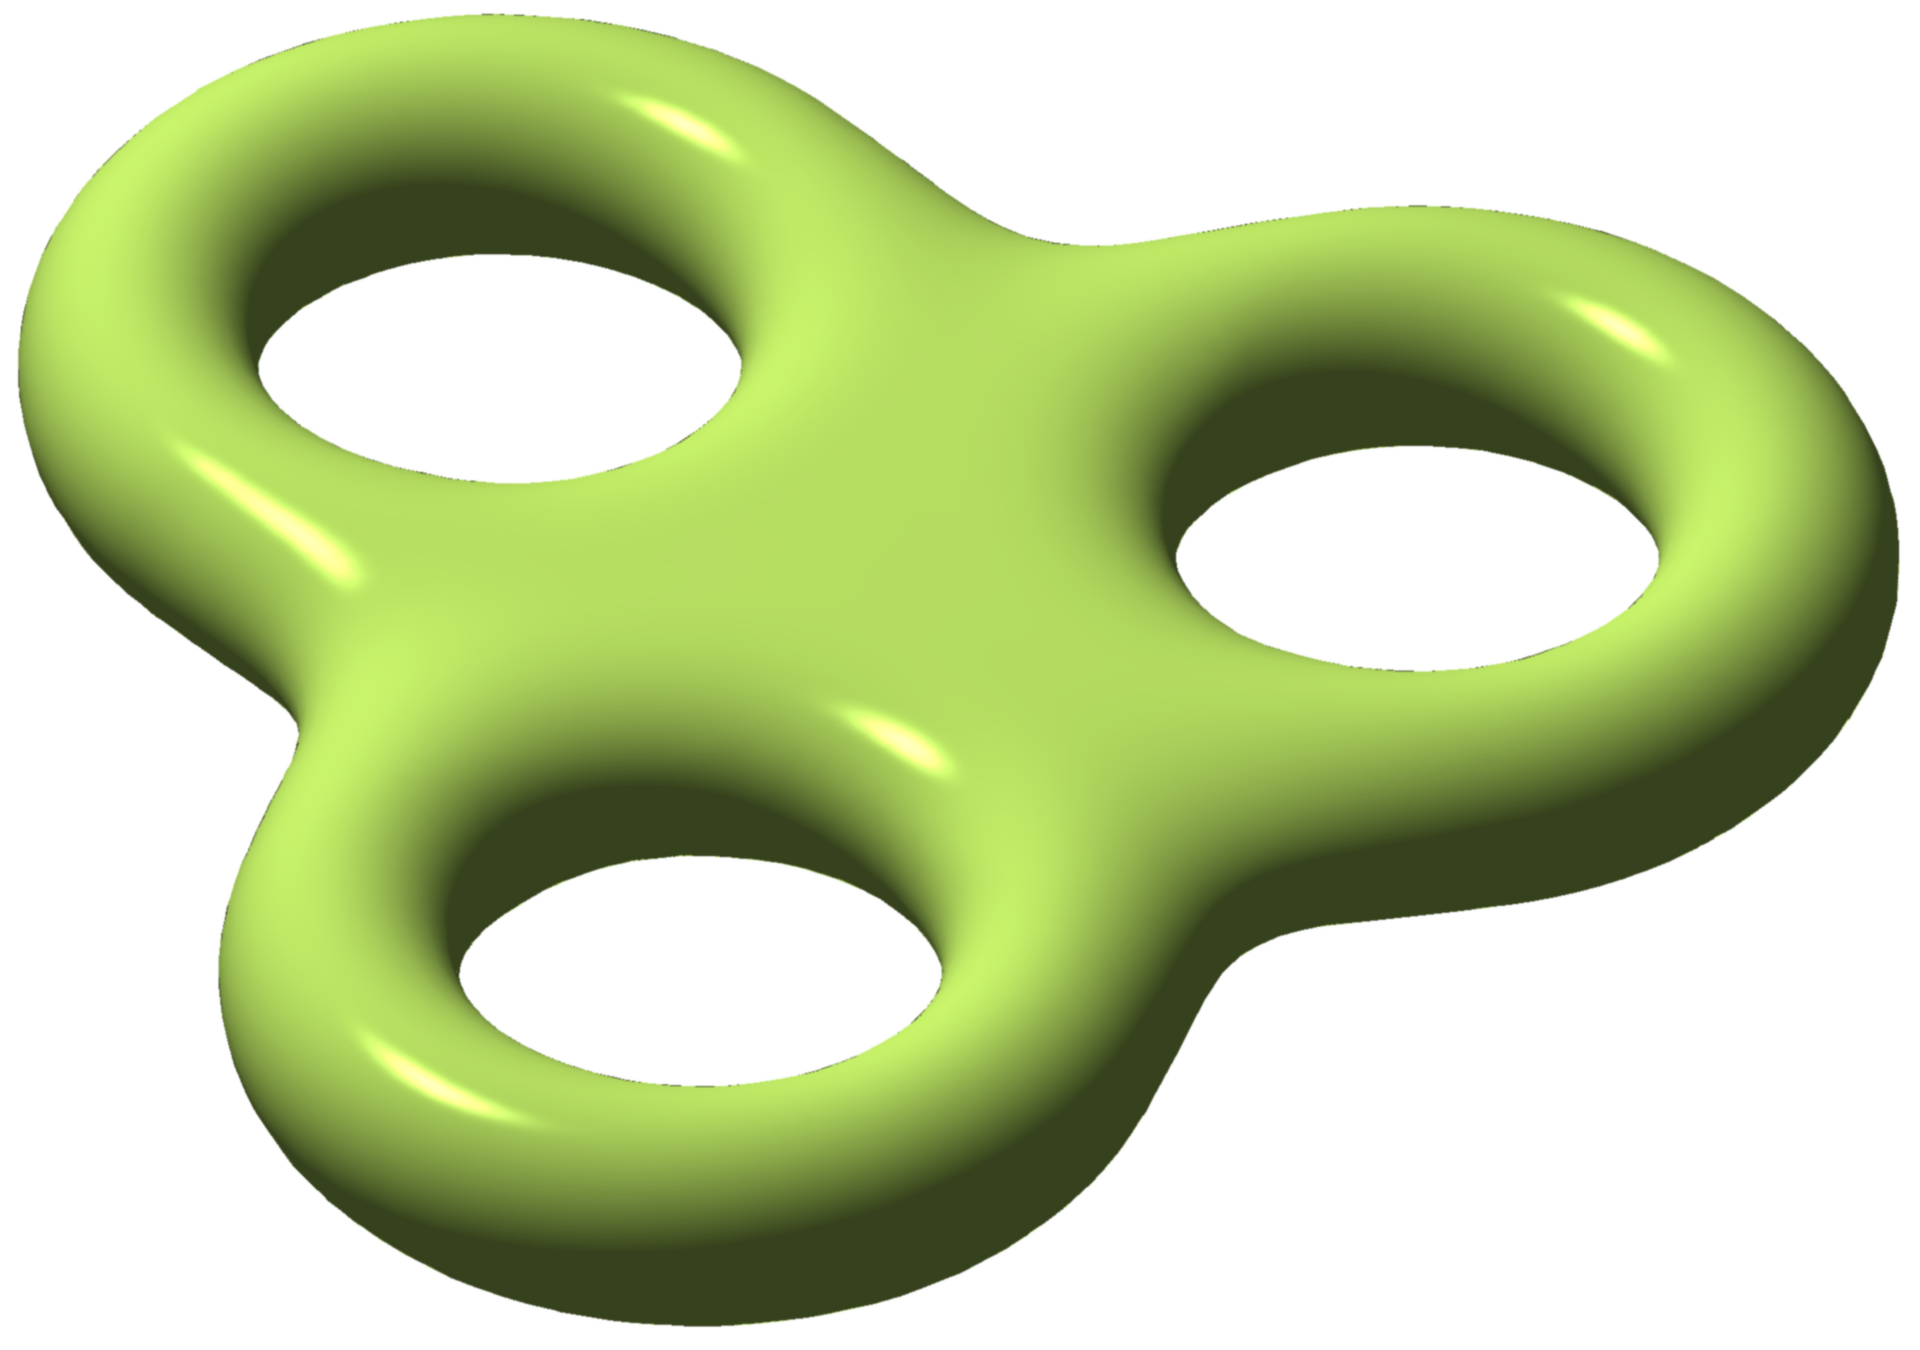
\includegraphics[scale = 0.5]{1920px-Triple_torus_illustration.png} 
        \caption{surfaces of genus two and three}
        \label{Fig3}
    \end{figure}

    With these graph theoretic and topological prerequisites we shall define the graph genus problem in section~\ref{sec2.1}. 

\section*{Genus of a graph}\label{sec2.1}
    Before we can go into the genus of the graph we shall first define what we mean by embedding a graph $G = (V, E)$ on a surface $X$.
    Embedding $G$ onto $X$ is drawing $G$ on $X$, such that no two edges of $G$ cross each other. 
    More formally our drawing is obtaining a subset $\Sigma$ of $X$ such that, for every vertex $v$ in $V$ we have a point $x$ in $\Sigma$ corresponding to $v$, 
    and for every edge $\{v,u\}$, if $x$ and $y$ are points in $\Sigma$ corresponding to $v$ and $u$ respectively then, there is a polygonal arc $p$ with endpoints $x$ and $y$, such that all $p \subseteq \Sigma$, and for each such $p$, $p\setminus\{x, y\}$ contains any point from any other polygonal arc or any point corresponding to a vertex.
    And finally, $G$ is isomorphic to the graph $\Sigma$. The regions of $X \setminus \Sigma$ are called the faces of $\Sigma$, intuitively these are the regions enclosed by the vertices and edges of $\Sigma$.

    Now we define what we mean by the genus of a graph. For a graph $G$ the genus $n$ of the surface $X$ with the smallest genus such that $G$ can be embedded on $X$ is called the genus of $G$. 
    It is denoted by $\gamma(G)$. For planar graphs the genus is 0, they can be embedded on a sphere, which minus its north pole is homeomorphic to a plane in $R^2$. For non-planar graphs, we will need surfaces of high genera.
    Figure~\ref*{Fig4} shows the embedding of $K_6$ (the complete graph with 6 vertices) on a torus.
    
    \begin{figure}[h]
        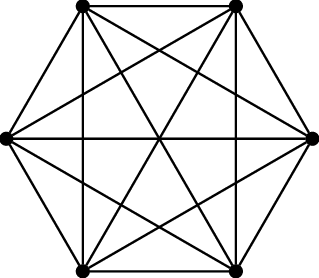
\includegraphics[scale = 0.5]{The-complete-graph-K-6.png} 
        \hspace*{1cm}
        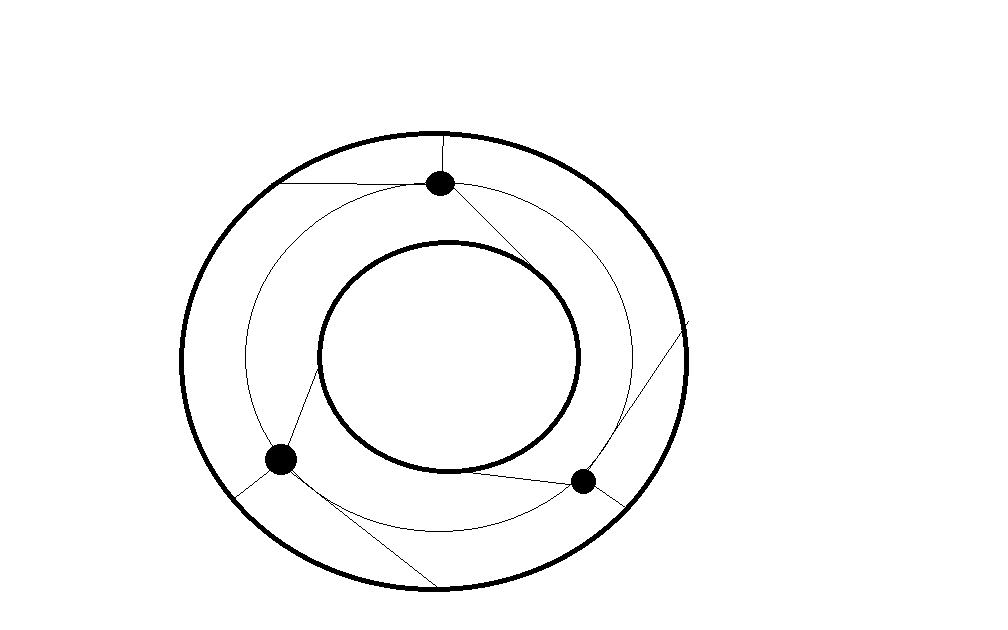
\includegraphics[scale = 0.4]{torus k6.png} 
        \caption{$K_6$ and its embedding on a torus, 3 vertices are placed on the top side of the torus and 3 are placed on the bottom of the torus.}
        \label{Fig4}
    \end{figure}

    Now the decision version of the graph genus problem is the following; GENUS = $\{\langle G = (V, E), k\rangle\mid \; \gamma(G) \leq k\}$.
    While the optimization version of the problem is; MIN-GENUS = $\{\langle G = (V, E), k\rangle\mid \; \gamma(G) = k\}$.
    So given a graph $G$ we need to find the genus of $G$. 

    For a long time, the complexity of GENUS was an open problem, in their book Garey and Johnson wrote it as one of the open problems in computational complexity theory \cite{GareyJohnson90}. 
    However, in 1989 Carsten Thomassen showed that GENUS was $\NPC$ \cite{Thomassen89}. He later in 1997 showed that it was $\NPC$ even when the input is restricted to cubic graphs \cite{Thomassen97}.
    While the optimization version of the problem MIN-GENUS is not even known to be in $\classNP$ and if $\NPH$. However, the problem has been shown to be fixed-parameter tractable as for any fixed genus there are only a finite number of forbidden graph minors \cite{Beyer16}, but for every surface, these are not known and finding the set of forbidden minors for a surface is not an easy task.
    So the problem remains one of the hardest problems in graph theory and algebraic topology.
    Furthermore, the problem has a higher complexity even for smaller graphs. The brute force approach run in $O(|V|^{\Delta(G)})$ time.

\section{Application of Genus problem}
    We now provide some application motivation for the graph genus problem.
    The utility problem is an infamous mathematical puzzle with numerous real-world applications. Kullman in his paper gives a comprehensive survey of the problem \cite{Kullman79}.
    According to Kullman, the problem dates back to ancient times, while the first published instance of the problem was given in 1917 by Henry Ernest Dudeney in his book Amusements in Mathematics \cite{Dudeney17, Kullman79}.
    The basic version of the problem is as follows, given three utilities, water, gas and electricity, and three houses A, B and C, on a street. 
    Now the task is to place the three utility connections to the three houses such that no connection crosses each other. For the three houses and utilities given in our example, the connections cannot be drawn on a plane.
    Figure~\ref*{Fig1} illustrates our example. Now we do however want to draw our connection, so maybe if we were given access to a tunnel we could pass some of our connections through it in order to solve the problem.
    For our example of three houses and three utilities only one such tunnel would be required. Now imagine we have some $n$ number of houses and $m$ number of utilities and now some houses might have some sort of connection to be built between them, or some utilities might need some connections between them.
    Now we need to know how many tunnels would be required to make our connections successfully
    So the problem becomes increasingly difficult. Another application of this problem comes in circuit embeddings. 
    When designing circuits we wish to embed on silicon chips we don't want different connections between our circuit components to cross. So our aim is to embed our circuit in such a that no connection crosses each other, it is of interest to us to find our how many holes do we need in order to successful embed the circuit.
    These real-world applications give us the motivation to define the graph genus problem. 
    % In section~\ref*{sec2} we shall give our problem definitions
    
    \begin{figure}[h]
        \centering
        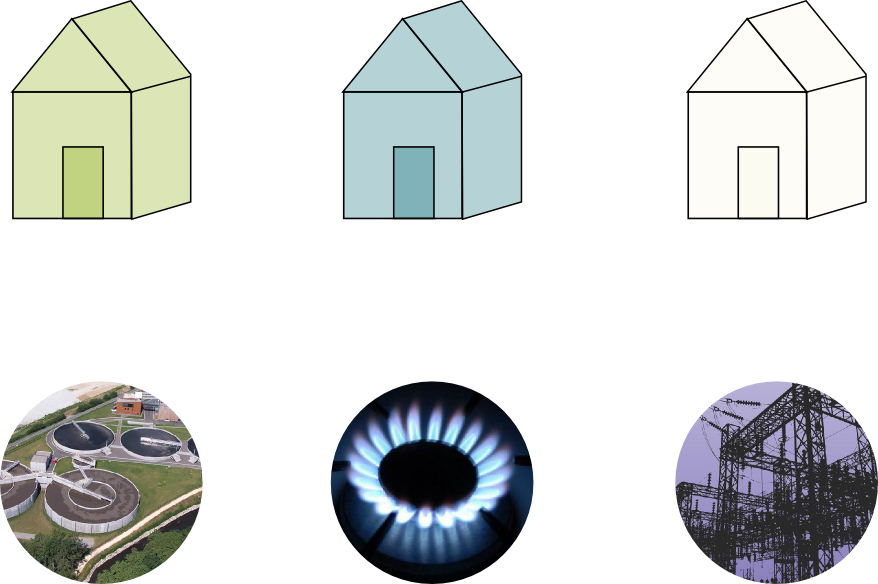
\includegraphics[scale = 0.2]{The-Utilities-Problem.png} 
        \hspace*{1cm}
        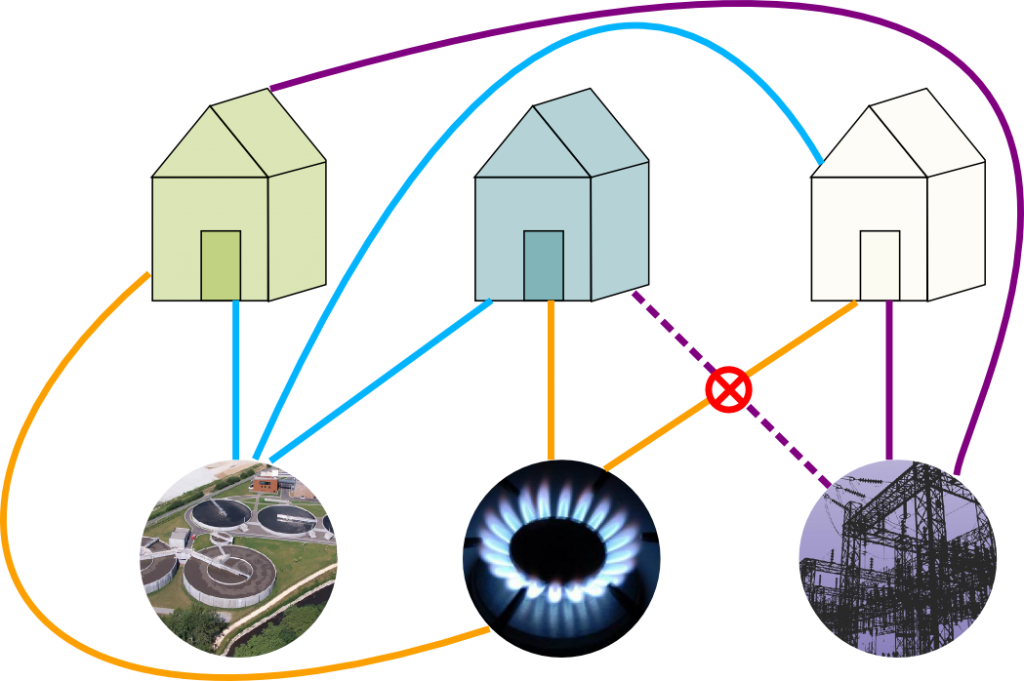
\includegraphics[scale = 0.2]{The-Utilities-Problem-Bad-Solution.png} 
        \caption{An illustration of utility problem}
        \label{Fig1}
    \end{figure}
    
\section{EA formulation}\label{sec: EA}

    As we saw the genus problem is quite a difficult problem to solve, and we have that no exact polynomial time solution exists for the problem unless $\classNP = \classP$.
    We would apply a meta-heuristic approach to solve the graph genus problem. More specifically we want to use an evolutionary algorithm to solve the graph genus problem.
    
    For this approach, it is of interest to us to formulate the problem as a combinatorial optimization problem. 
    Throughout history, many such approaches have been made most famously the formulation given by Filotti in 1979 \cite{Filotti79}. However Wendy Myrvold and William Kocay showed that there is a flaw in the formulation by Filotti, they also identified errors in many famous algorithms which try to solve the graph genus problem \cite{Myrvold11}.
    However many other valid formulation exists, for example, the formulation given by G. Brinkmann \cite{brinkmann20}, Marston Conder and Klara Stokes \cite{Conder19}, Stephan Beyer and Markus Chimani and Ivo Hedtke and Michal Kotrbcik \cite{Beyer16}, among others.
    
    For our approach, we solely consider combinatorial embeddings. For a graph $G = (V, E)$
    A combinatorial embedding is given by a rotation system $R$ defined on $G$.

\section{Experimental Evaluation}\label{sec: exp}

\section{Conclusion}\label{sec: con}


% \section{Problem statement}\label{sec3}
%     As we saw the genus problem is quite a difficult problem to solve, and we have that no exact polynomial time solution exists for the problem unless $\classNP = \classP$.
%     We would apply a meta-heuristic approach to solve the graph genus problem. More specifically we want to use an evolutionary algorithm to solve the graph genus problem.
    
%     For this approach, it is of interest to us to formulate the problem as a combinatorial optimization problem. 
%     Throughout history, many such approaches have been made most famously the formulation given by Filotti in 1979 \cite{Filotti79}. However Wendy Myrvold and William Kocay showed that there is a flaw in the formulation by Filotti, they also identified errors in many famous algorithms which try to solve the graph genus problem \cite{Myrvold11}.
%     However many other valid formulation exists, for example the formulation given by G. Brinkmann \cite{brinkmann20}, Marston Conder and Klara Stokes \cite{Conder19}, Stephan Beyer and Markus Chimani and Ivo Hedtke and Michal Kotrbcik \cite{Beyer16}, among others.
    
%     The formulation of interest to us is the one by Stephan Beyer .et al \cite{Beyer16}. Stephan Beyer gave two formulation of the problem of computing the number of faces in a valid embedding on a graph $G$ on surface $X$ of genus $g$, the first formulation, formulates the problem as a Boolean satisfiability problem.
%     A boolean formula $\phi$ is called satifiable if there is a truth assignment of the variables of $\phi$ such that $\phi$ evaluates to true.
%     The formulation constructs a boolean formula from the graph and a given number of faces $f$. The formula is satifiable if and only if we have that an embedding of $f$ faces exits for $G$. The over formulation is of more interest to us. 
%     The second formulation, formulates the problem as an integer linear program problem. The program is constructed from the input graph.
%     The objective function is to maximize the number of faces. The detailed problem formulation is as follows:
%     Let $G = (V, E)$ be a graph, let $A = \{(u, v), (v, u) | {u,v} \in E\}$ here is the set of two directed edges for each edge in $E$.
%     Let $\overline{f}$ be an upper bound on number of faces, for each $i \in \overline{f}$, we have a binary variable $x_i$ that is
%     1 if and only if the $i^{\text{th}}$ face exists in a embedding of $G$, and we have a binary variable $c_a^i$, for each $a \in A$, that is 1
%     if and only if polygonal arc $a$ (corresponding to some edge $e$) is on the boundary of $i^{\text{th}}$ face. 
%     For each vertex $v \in V$ and neighbors $u, w \in N(v)$ such that $u \neq w$, we have a binary variable $p^v_{u,w}$, which is 1 if and only if $w$ is a successor of $u$ in rotation at $v$. So now the integer linear program formulation is as follows:
%     \\$\displaystyle{\text{max } \sum^{\overline{f}}_{i = i} x_i, \text{ such that,}}$
%     \begin{enumerate}
%         \item $\forall i \in \overline{f},\; x_i  \leq \frac{1}{3}\sum_{a \in A} c^i_a$
%         \item $\forall a \in A,\; \frac{1}{3}\sum_{i = 1}^{\overline{f}} c^i_a = 1$
%         \item $\forall i \in \overline{f} \;\forall v \in V,\; \sum_{a \in d^+(v)} c^i_a = \sum_{a \in d^-(v)} c^i_a$
%         \item $\forall i \in \overline{f} \;\forall v \in V,\; u,w \in N(v), s.t\; u \neq w,\; c^i_{vw} \geq c^i_{uv} + p^v_{u,w} - 1$
%         \item $\forall i \in \overline{f} \;\forall v \in V,\; u,w \in N(v), s.t\; u \neq w,\; c^i_{uv} \geq c^i_{vw} + p^v_{u,w} - 1$
%         \item $\forall v \in V, u \in N(v), \; \sum_{w \in N(v), u \neq w} p^v_{u, w} = 1$
%         \item $\forall v \in V, w \in N(v), \; \sum_{w \in N(v), u \neq w} p^v_{u, w} = 1$
%         \item $\forall v \in V, \emptyset \neq U \subseteq N(v), \; \sum_{u \in U}\sum_{w \in N(v)\setminus U} p^v_{u, w} \geq 1$
%         \item $\forall i \in \overline{f},\; x_i  \in \{0,1\}$
%         \item $\forall i \in \overline{f},\; \forall a\in A,\; c_a^i  \in \{0,1\}$
%         \item $\forall v \in V,\; u,w \in N(v), s.t\; u \neq w,\; p^v_{u, w}  \in \{0,1\}$
%     \end{enumerate}
%     Now the problem is finding satisfying assignment of $x_i$, $c_a^i$, and $p^v_{u, w}$, $\forall i \in \overline{f} \; \forall i \in \overline{f},\; \forall a\in A, \; \forall v \in V,\; u,w \in N(v), s.t\; u \neq w$ such that $\sum^{\overline{f}}_{i = i} x_i$ is maximized.
%     Now the number of faces we compute through this formulation connects beautifully the genus of the graph, by the following equation $2 - 2\gamma(G) = |V| - |E| + f$ \cite{Massey91}.
%     Through this once we have maximize the number of faces we can compute the minimum genus of the graph.
    
%     Now we will use a meta-heuristic approach to minimize the number of faces in the integer linear program formulation of the graph genus problem. We will use an evolutionary algorithm to minimize the number of faces in the embedding of $G$ computed from the integer linear program formulation.
%     Through this we compute the minimum genus of the graph. We will implement our algorithm in python and test our approach on various different graphs with known genera.

\bibliographystyle{plain} 
\bibliography{ref}


\end{document}

